\documentclass[../main.tex]{subfiles}
\usepackage{graphicx}
\usepackage{subcaption}
\usepackage{adjustbox}

\begin{document}
\subsection{Procedimiento para la calibración de resortes}
\begin{enumerate}
  \item Pesar las masas de las pesas en una balanza digital para
  obtener su incertidumbre luego pasaremos a enumerar cada pesa.
  \item Colocar una marca a cada resorte (A y B) para distinguirlos y 
  luego medir Su longitud natural(sin elongar) para ver quien es el resorte mas largo y el mas corto .
  \item Fijar un extremo del resorte A al soporte universal y al otro extremo 
  le pondremos la pesa numero uno  una vez en equilibrio con una regla pasaremos a medir la elongación para restarle su longitud natural , este procedimiento lo realizaremos muchas veces formando combinaciones sin quitar la pesa numero uno , el mismo procedimiento lo realizaremos con el resorte B .
  \item Estos datos serán anotados en una hoja de apunte.
\end{enumerate}

\begin{figure}
  \centering
  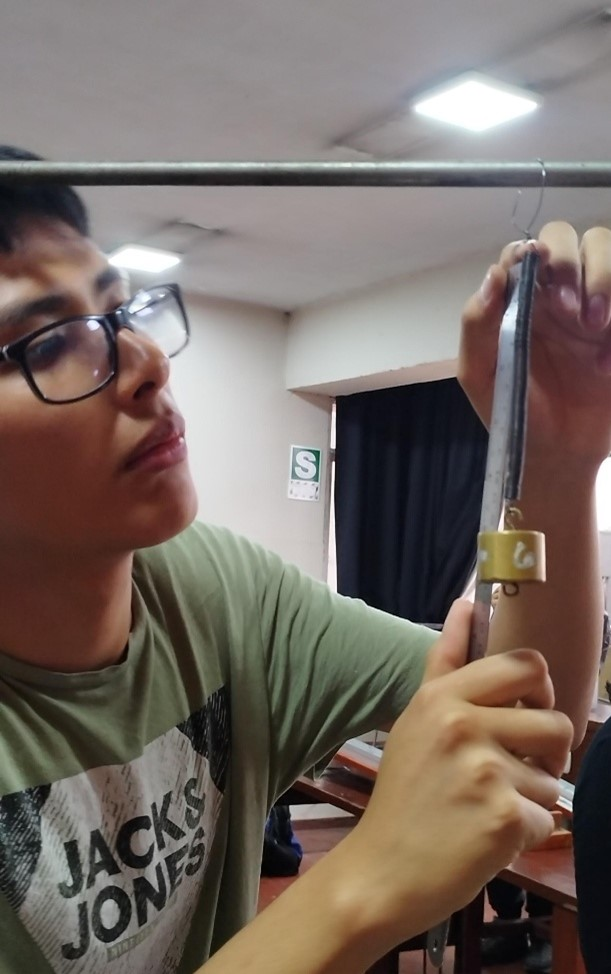
\includegraphics[width=0.4\linewidth]{images/proc3.jpg}
  \caption{Proceso de la calibración de los resortes.}
  \label{fig:proc3}
\end{figure}

\subsection{Procedimiento para la obtención de la trayectoria del disco}
\begin{enumerate}
  \item Nivelar horizontalmente la plataforma de vidrio utilizando los tornillos y el nivel.
  \item Colocar y centrar el pliego de papel encima de la plataforma.
  \item Posicionar los resortes con un extremo en cada gancho asignado y otro en el mango del disco.
  \item Marcar en el papel las posiciones A y B de los puntos fijos de los resortes.
  \item Configurar el chispero para utilizar frecuencia de 20 Hz.
  \item Permitir el flujo de aire hacia el disco para eliminar la fricción con el papel.
  \item Practicar el posicionamiento del disco hasta que, consistentemente, al soltarlo su trayectoria cruce consigo misma una vez.
  \item Marcar la posición inicial elegida como 0.
  \item Soltar el disco desde la posición 0 en sincronía con el encendido del chispero y apagar el chispero cuando el lazo de la trayectoria esté completo.
  \item Repetir según sea necesario para obtener marcas satisfactorias en el papel.
\end{enumerate}

\begin{figure}[H]

  \begin{tabular}{c c}
      
  \begin{subfigure}{0.5\textwidth} 
      \centering
      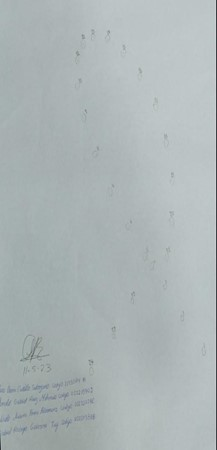
\includegraphics[width=0.4\linewidth,angle=90]{images/proc1.jpg}
      \caption{Forma de e obtenida en el papel.}
      \label{fig:e}
  \end{subfigure}
  &
  \begin{subfigure}{0.5\textwidth}  
      \centering
      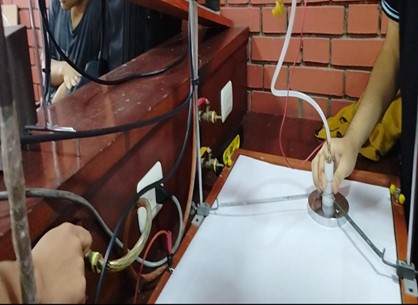
\includegraphics[width=0.8\linewidth, height=3.5cm]{images/proc2.jpg}
      \caption{Tablero preparado con el disco metálico.}
      \label{fig:proc_disco}
  \end{subfigure} \\
  \end{tabular}
  
  \caption{Imágenes del proceso de la obtención de la trayectoria del disco.}
  \label{fig:proc}
\end{figure}

\end{document}